\section{Advanced Hardware Construction in Chisel}
Another way to support hardware facilities in Chisel, as opposed to
building new nodes, is to write a Scala program that aggregates the
features of Chisel from Chapter~\ref{sec:chisel} into a directed graph
of nodes that implement the same hardware functionality. This approach
has the advantage of decoupling the hardware facility from the
backend, making the hardware facility more accessible as it can now be
mapped to more backends. The only requirement on the backend is that
they can support the basic Chisel nodes from
Chapter~\ref{sec:chisel}. Furthermore, the designer is no longer
required to write the code generation function for every single
backend, saving a great deal on designer effort. The rest of this
chapter will show how to implement ListLookup and Vec using only the
basic Chisel nodes presented in Chapter~\ref{sec:chisel}

\subsection{ListLookup}
\begin{figure}[htb]
\centering
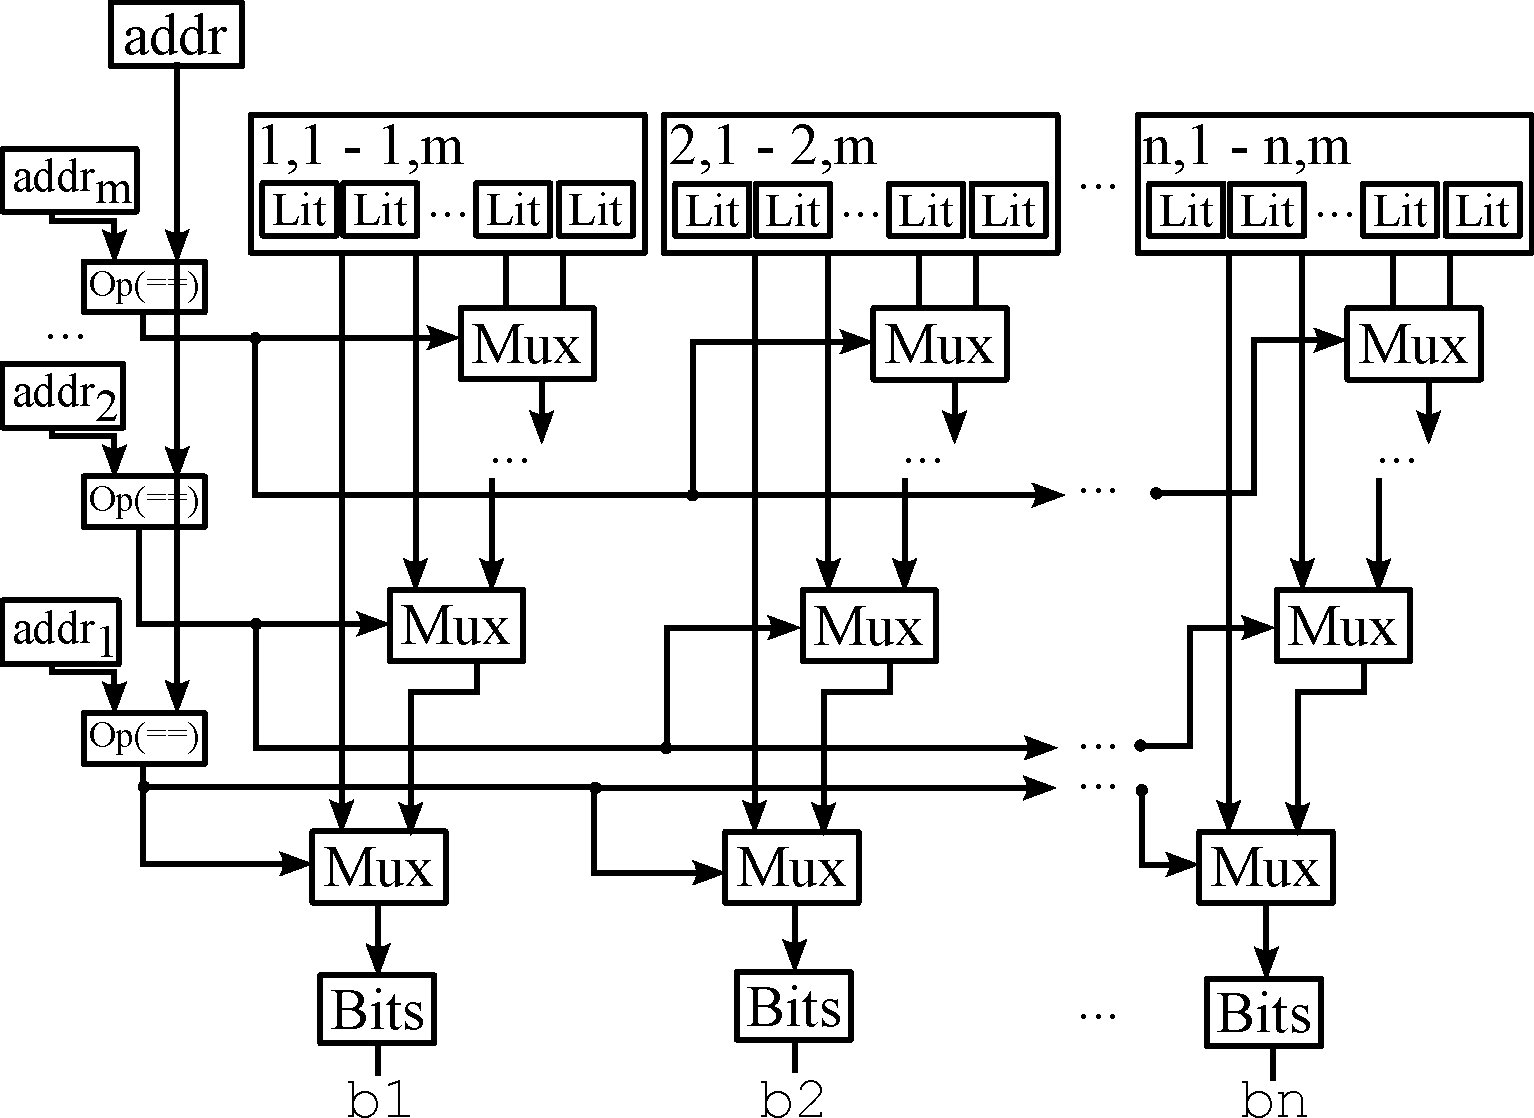
\includegraphics[width=0.7\textwidth]{figures/listlookupscala.pdf}
\caption{ListLookup implemented using Scala code and basic Chisel nodes}
\label{fig:llscala}
\end{figure}

The syntax for ListLookup remains the same. Users provide an address
for lookup and a list of size $m$ of tuples {\tt ($a_i$, $lits_i$)}
where {\tt $a_i$} is the address to match the lookup address against and
{\tt $lits_i$} is a list of size $n$ of literals to return when there
is a match. The ListLookup will then construct the graph in
Figure~\ref{fig:llscala}. The function returns a list of {\tt Bits}
{\tt $b_1$, ... $b_n$} who will take on the values of {\tt $lits_i$} if
{\tt $a_i$} matches the lookup address.

ListLookup graphs are constructed as follows. Given the input list of
tuples {\tt ($a_i$, $lits_i$)}, create $n$ list of $m$ tuples
{\tt $( (a_1, l_{1, k}), ... (a_j, l_{j, k}), ..., (a_m, l_{m, k})
  )$}. Each of these list represents a mux chain and there are $n$
such list ($k$ ranges from 1 to $n$). The mux chains are constructed
using {\tt $a_i$ === addr} as the select signal to the corresponding
mux. If the address matches, then literal {\tt $l_{i, k}$} is outputted
for Bits $b_k$.

\subsection{Vec}
\begin{figure}[htb]
\centering
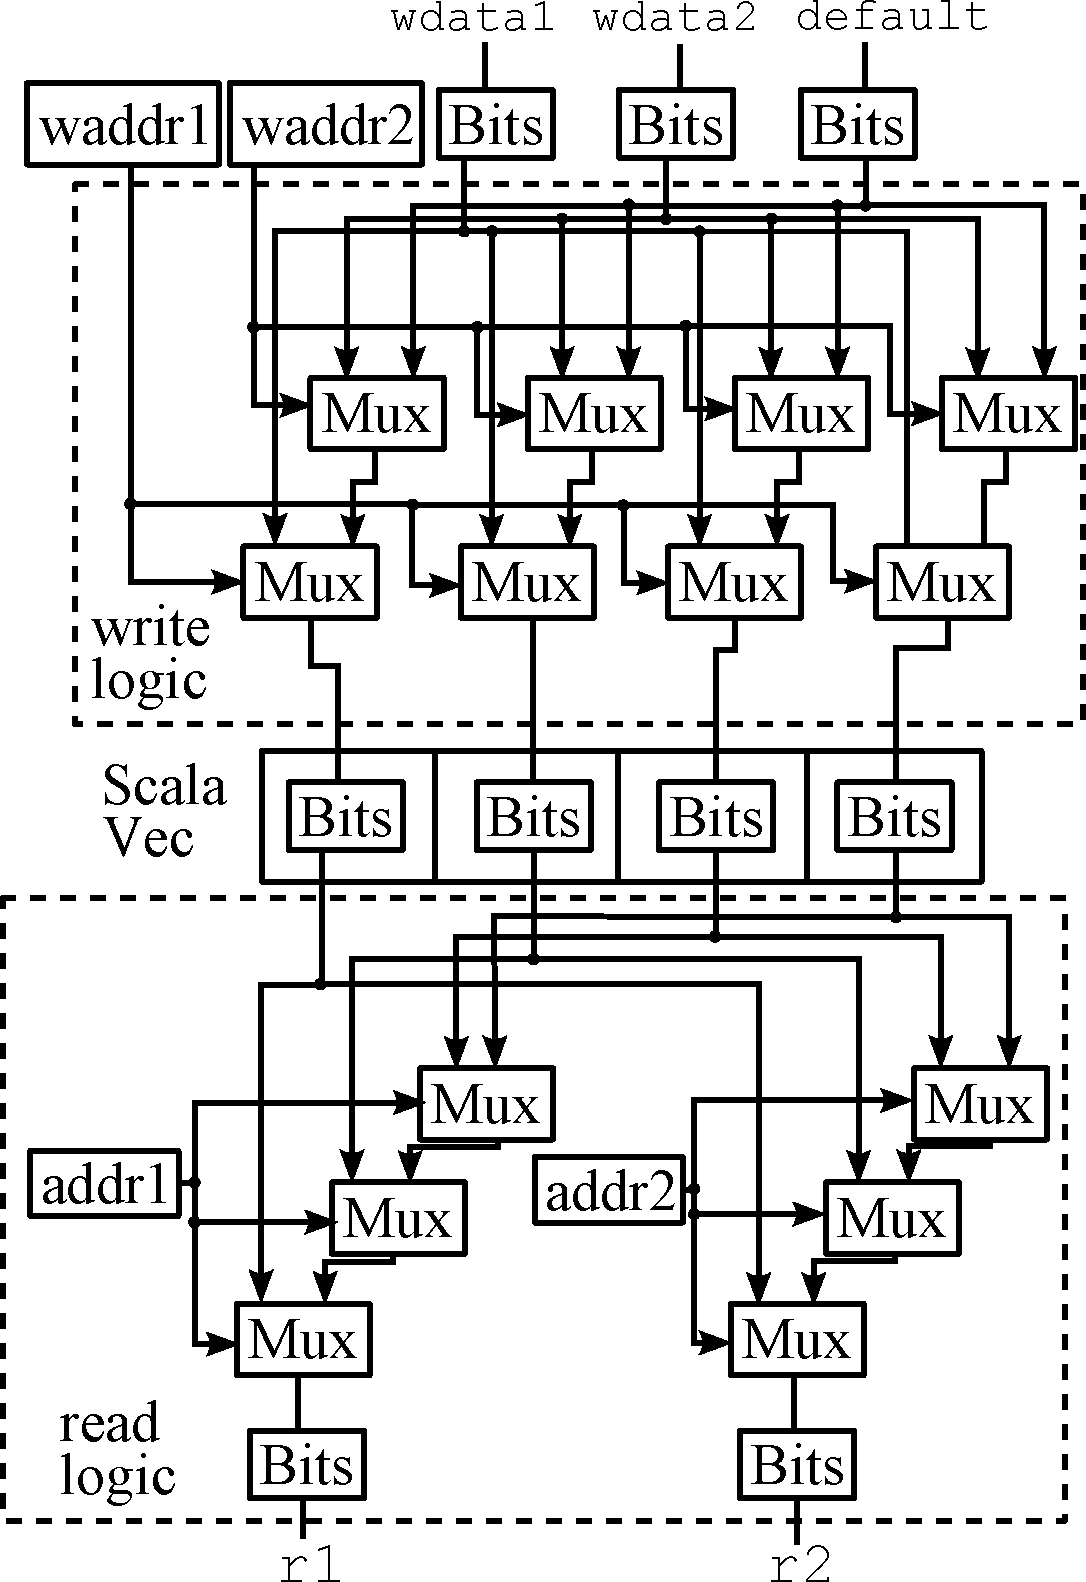
\includegraphics[width=0.5\textwidth]{figures/vecscala.pdf}
\caption{Vec implemented using Scala code and basic Chisel nodes}
\label{fig:vecscala}
\end{figure}

Figure~\ref{fig:vecscala} shows the resulting graph from building a
Vec using only basic Chisel nodes. Note that Vec is now a Scala array
of {\tt Bits} and is not a {\tt Node}. The syntax for constructing a
Vec is unchanged; users instantiate the Vec with the desired
size. Since the Vec is now a Scala array, users populate the Vec using
Scala array syntax, e.g.
\begin{align*}
  \text{ \tt{v(1) = Bits(width=32)} }
\end{align*}
where {\tt v} is the name of the Vec. The syntax for reading and
writing to the Vec is also unchanged. The difference is that reads
and writes will now construct the graph in Figure~\ref{fig:vecscala}
instead of instantiating special read and write nodes.

\textbf{Reads} A Vec can be indexed with either Scala integer or a
Chisel {\tt Node}. If a Scala integer is used, no {\tt Nodes} are
created and the element at that index is returned. If a Chisel 
{\tt Node} is used, then a Mux chain is built to mux out the correct
element of the Vec. The select signal to the mux is {\tt addr === idx}
where {\tt addr} is the address and {\tt idx} ranges from zero to
length of the Vec minus 1. When {\tt addr} matches an {\tt idx}, the
element at {\tt v(idx)} is outputted.

\textbf{Writes} Like reads, a Vec can be written to using either a
Scala integer or a Chisel {\tt Node} for indexing. If a Scala integer
is used, then the corresponding element is accessed and written to and
no nodes are constructed. If a Chisel {\tt Node} is used, then a mux
is placed in front of each element in the Vec. The select signal to
the mux is {\tt waddr ==== idx} where {\tt waddr} is the input write
address and {\tt idx} ranges from zero to the length of the Vec minus
1. If the write address matches the {\tt idx}, then the element at
{\tt v(idx)} is written to with the write data, otherwise {\tt v(idx)}
is written to with the default data. If the {\tt Vec} contains 
{\tt Bits} then the user supplies the default data. If the {tt Vec}
contains {\tt Reg} nodes then no default signal is needed.
